\documentclass[10pt]{article}

\usepackage{microtype}
\usepackage{graphicx}
\usepackage{times}
\usepackage{natbib}
\usepackage{amsmath,amssymb}
\usepackage{hyperref}
\usepackage{booktabs}
\usepackage{multicol}
\usepackage{siunitx}
\usepackage{float}
\usepackage{multicol}
\usepackage{multirow}

\setlength{\textwidth}{6.75in}
\setlength{\textheight}{9.0in}
\setlength{\columnsep}{0.25in}
\setlength{\topmargin}{-0.5in}
\setlength{\oddsidemargin}{-0.25in}
\setlength{\evensidemargin}{-0.25in}

\begin{document}

\title{Neural Networks Learn Distance Metrics}
\author{Alan Oursland\\
Independent Researcher\\
\texttt{alan.oursland@gmail.com}}
\date{January 2025}

\maketitle

\begin{abstract}
    Neural networks have historically relied on intensity-based representations, where larger activations indicate stronger feature presence. Recent theoretical work, however, suggests that distance-based representations—where smaller activations signify stronger feature matches—may naturally emerge in hidden layers. This paper systematically investigates neural network feature learning through six architectural variants, revealing that networks naturally learn statistical distance metrics, with their success determined by how effectively they can represent and leverage these distance-based features. We provide theoretical and empirical insights into why certain architectures catastrophically fail under intensity constraints (47.20\% accuracy) while others maintain robust performance (95.35\% accuracy). To address these challenges, we introduce \textit{OffsetL2}, a novel architecture explicitly integrating Mahalanobis distance computations. OffsetL2 achieves remarkable performance and stability for such a small model, attaining 97.61\% accuracy on MNIST with minimal variance ($\pm$0.07\% standard deviation). These results validate our geometric framework and underscore the potential of explicitly modeling statistical distance measures in neural architectures to enhance performance and interpretability.

\end{abstract}
    
\begin{multicols}{2}  % Start two columns without page break

\section{Introduction}

Neural networks have revolutionized machine learning through their ability to learn complex internal representations. While early models like the McCulloch-Pitts neuron conceptualized neural activations in intensity-based terms (larger activation indicating stronger feature presence), recent theoretical work suggests that distance-based interpretations may arise naturally in hidden layers. This tension between distance-based and intensity-based representations has significant implications for network design, optimization, and interpretability.

\subsection{The Core Question}

A fundamental question emerges: Do neural networks inherently favor distance-based or intensity-based representations? In distance-based encoding, smaller activations indicate stronger matches to learned prototypes, mathematically expressed as:

\begin{equation}
    a(x) = \|W(x - \mu)\|_p
\end{equation}

where $\mu$ represents a learned prototype and $W$ a scaling matrix. Conversely, intensity-based encoding treats larger activations as indicating stronger feature presence:

\begin{equation}
    a(x) = f(Wx + b)
\end{equation}

where $f(\cdot)$ is an activation function applied to an affine transformation.

\subsection{Implications and Applications}

Understanding these representational biases is critical for:

\begin{itemize}
    \item Designing robust and interpretable networks that naturally align with distance-like encodings.
    \item Explaining catastrophic failures in certain architectures under intensity-based assumptions.
    \item Informing practical design choices, such as activation functions, normalization schemes, and bias terms.
\end{itemize}

\subsection{Our Contribution}

This paper systematically investigates representational biases in neural networks and offers the following contributions:

\begin{enumerate}
    \item A controlled experimental study comparing six architectural variants, revealing how geometric constraints shape internal representations.
    \item A novel analysis connecting representational biases to the geometric properties of feature spaces.
    \item Development of OffsetL2, an architecture that explicitly incorporates Mahalanobis distance calculations, achieving improved performance and stability across tasks.
\end{enumerate}

Our findings demonstrate that the success or failure of neural architectures is not dictated by an inherent bias toward distance or intensity representations but by their interaction with the geometric constraints of the feature space. OffsetL2 exploits these geometric principles, achieving significant performance gains, including a $<specific result here>$. This work provides a robust framework for understanding and optimizing representation learning, with applications to classification, clustering, and beyond.

\section{Related Work}
\label{sec:related_work}

Interpreting neural network representations through distance metrics offers a promising avenue for enhancing their interpretability and robustness. Our recent theoretical work has established a fundamental connection between neural network computations and statistical distance measures like the Mahalanobis distance \cite{mahalanobis1936generalized}. We demonstrated how linear layers with Absolute Value (Abs) activations can approximate the Mahalanobis distance, suggesting that neural networks may learn to represent data in terms of distances to learned prototypes \cite{oursland2024interpreting}. We further supported this theoretical framework with empirical evidence showing that neural networks with ReLU and Abs activations are more sensitive to perturbations that modify distance relationships in the feature space than to those that merely alter activation magnitudes \cite{oursland2024neural}. 

Alternative approaches, including Radial Basis Function (RBF) networks \cite{broomhead1988rbf}, Siamese networks \cite{bromley1994signature}, and Learning Vector Quantization (LVQ) \cite{kohonen1995learning}, have explored the explicit integration of distance metrics into neural architectures, primarily for clustering and metric learning tasks. Prototype-based models, which learn representations of classes and classify inputs based on their proximity to these prototypes, also implicitly rely on distance computations \cite{snell2017prototypical}. While these methods demonstrate the potential of distance-based learning, they have not seen widespread adoption in general-purpose deep learning architectures.

Complementing these distance-centric views, geometric interpretations of neural computation offer valuable perspectives for understanding internal representations \cite{montavon2018methods, samek2019explainable}. These approaches often analyze hyperplanes and decision boundaries to explain how networks partition and represent data. However, while providing valuable insights into network behavior, these studies often focus on networks trained under standard intensity-based assumptions. This work aims to bridge the gap between distance-based and geometric interpretations by investigating how architectural choices, such as activation functions and the explicit incorporation of distance metrics, influence the emergence of distance-based representations and shape the geometry of the learned feature space.


\section{Background}
\label{sec:background}

This section introduces the theoretical framework for understanding how neural networks represent data through either distance-based or intensity-based methods, providing context for our experimental analysis.

\subsection{Features, Representations, and Distance Metrics}

Neural networks learn features through their internal representations. For the purposes of this paper, we define \textbf{features} as inherent properties of the data that can be quantified statistically, and \textbf{representations} are the compositions of these features learned by a node to generate its output. Traditional intensity-based representations encode features through activation magnitudes, while distance-based representations encode features through proximity to learned prototypes. In our discussion, we primarily consider prototypes as the features of interest, as they provide a structured way to quantify similarity and influence learned representations.

We argue that neural networks fundamentally learn distance features that quantify similarity between data points and learned prototypes. What appear to be intensity-based representations can be reinterpreted as disjunctive sets of distance features, corresponding to Disjunctive Normal Form (DNF) in Boolean algebra \cite{post1921introduction}. For example, an intensity representation for class $a$ implicitly learns $\lnot(b \lor c) = \lnot b \land \lnot c$, where $b$ and $c$ represent distances to other classes. This logical interpretation has connections to work exploring the relationship between neural networks and Boolean formulas \cite{anthony2003boolean}

In contrast, distance-based representations directly encode proximity to prototypes as conjunctive sets (Conjunctive Normal Form). For class $a$, this simply requires a small distance to prototype $a$, represented logically as $a$. This more directly captures the underlying statistical relationships in the data.

\subsection{Distance vs. Intensity Representations}
\label{subsec:dist-intensity-rep}

Intensity-based interpretations, while lacking precise mathematical definition, are deeply embedded in the foundations of deep learning \cite{goodfellow2016deep}. These interpretations treat larger activations as indicating stronger feature presence, fundamentally shaping how we train and interpret networks. The use of one-hot encoded labels for classification directly encodes this assumption - the correct class should produce the highest activation while all others should be suppressed. This intensity-based paradigm appears throughout modern practice: cross-entropy loss encourages larger activations for correct classes, feature visualization \cite{erhan2009visualizing, olah2017feature} assumes maximum activations represent learned features, and even basic image processing interprets pixel intensities as direct measures of feature strength. However, this pervasive intensity-based interpretation remains an assumption imposed on neural networks rather than an inherent property.

Distance-based representations offer an alternative framework, interpreting smaller activations as indicating similarity to learned prototypes. This aligns with statistical metrics like the Mahalanobis distance \cite{mahalanobis1936generalized}, where the activation $f(x)$ is inversely proportional to the distance between input $x$ and prototypes $\mu$:

\begin{equation}
f(x) = |W(x - \mu)|_p,
\end{equation}

where $W$ is a learned scaling matrix and $p$ denotes the norm. Common activation functions naturally support this view: the absolute value function directly represents distance, while ReLU implicitly encodes distance through the relationship $Abs(x) = ReLU(x) + ReLU(-x)$. This framework emphasizes geometric relationships in the latent space rather than activation magnitudes. This perspective aligns with research on visualizing and understanding the loss landscape of neural networks \cite{li2018visualizing, goodfellow2015qualitatively}.

\subsection{Theoretical Foundations: Mahalanobis Distance}

The Mahalanobis distance provides a statistical foundation for distance-based representations, capturing feature correlations and scales through the covariance matrix $\Sigma$:
\begin{equation}
    D_M(x) = \sqrt{(x - \mu)^T \Sigma^{-1} (x - \mu)},
\end{equation}

Through eigendecomposition $\Sigma = V\Lambda V^T$, this distance can be expressed as:
\begin{equation}
    D_M(x) = \| \Lambda^{-1/2} V^T (x - \mu) \|_2,
\end{equation}
revealing how neural networks naturally approximate this metric: linear layers weights learn the eigenvector transformation $\Lambda^{-1/2} V^T$, the bias learns $-\Lambda^{-1/2} V^T \mu$, and activation functions like Absolute Value model the normalized distance computation \cite{oursland2024interpreting}.

\subsection{Geometric Interpretations of Representations}

Neural networks project input data into a latent space structured by hyperplanes; under a distance-based interpretation, these hyperplanes act as axes of a manifold, with distances to prototypes along these axes defining the representation \cite{montavon2018methods}.

For a hyperplane defined by $y = Wx + b$, where $x$ is $N$-dimensional and $y$ is scalar, its decision boundary occurs where the activation function equals zero (e.g., $0 = Wx + b$). This boundary is uniquely described by $N$ linearly independent points: $N-1$ points on the decision boundary plus one point at ${x=0, y=b}$. These boundary points serve as feature prototypes, encoding relationships between inputs and their latent representations. These prototypes don't necessarily reflect human-perceived similarity, but rather capture relationships defined by the network's learned distance metric.

When $b=0$, hyperplanes must pass through the origin, making it a fixed prototype. This constraint has minimal impact in high dimensions since each hyperplane still intersects $N-2$ independent points on its decision boundary, plus points at the origin and ${x!=0, y!=0}$. While these prototypes are theoretically significant, recovering them becomes computationally intractable as dimensionality increases \cite{donoho2000high}.

\subsection{Activation Functions and Representational Preferences}

Activation functions shape how networks encode representations:

\begin{itemize}
    \item \textbf{ReLU}: $f(x) = \max(0, x)$ is traditionally associated with intensity-based interpretations but can be viewed through a distance lens \cite{nair2010relu, glorot2011deep}. The zero region corresponds to one side of a decision boundary, with positive activations encoding prototype proximity. However, ReLU's tendency to produce "dead neurons" when inputs remain negative can hinder learning. This issue has motivated research into alternative activation functions \cite{he2015delving, ramachandran2017searching, misra2019mish}.
    
    \item \textbf{Absolute Value (Abs)}: $f(x) = |x|$ directly represents distance-based relationships by preserving magnitude information regardless of sign. This symmetry ensures neurons remain active and maintain complete information about distance from decision boundaries.
    
    \item \textbf{Neg Layers}: $f(x) = -x$ transform positive distance representations into negative intensity representations by inverting activation order.
\end{itemize}

This theoretical foundation frames our experimental analysis, where we systematically investigate how architectural choices, such as activation functions and bias terms, affect representational biases. By probing these factors, we aim to elucidate the fundamental principles driving neural network learning and provide a unified framework for understanding distance-based and intensity-based representations.

\section{Experimental Design}
\label{sec:exp_design}

This experimental design aims to investigate how different architectural constraints influence the learning dynamics and representational biases of neural networks. Specifically, we explore whether networks exhibit a preference for distance-based or intensity-based representations when learning features from data. By systematically varying key architectural components, such as activation functions and the presence or absence of bias terms, we aim to gain empirical insights into the interplay between network architecture, learned representations, and the underlying geometry of the feature space. The results will inform our understanding of whether neural networks fundamentally learn distance metric features, and how architectural choices might facilitate or hinder the development of such representations.

\subsection{Objectives}
Our experiments address the following key questions:
\begin{enumerate}
    \item When neural networks are constrained to produce either distance-based or intensity-based outputs, how does this affect their overall performance and learning dynamics?
    \item How do different activation functions and the presence or absence of bias terms in the output layer influence the network's ability to learn under these different representational constraints?
    \item By analyzing the performance and behavior of networks under these constraints, what can we infer about the nature of the representations learned in the hidden layer and the geometry of the feature space?
\end{enumerate}

\subsection{Architectural Variants}To investigate how different output constraints affect network learning and the resulting representations, we employ six two-layer architectures. These architectures are intentionally kept simple to isolate the specific behaviors under study. They systematically vary key components: the choice of activation function, the presence of a negation operation at the output, and the use of a bias term in the final linear layer. The rationale behind these choices is as follows:

\begin{enumerate}
    \item \textbf{Two-layer Networks}: We utilize two-layer networks for their simplicity and widespread use in fundamental studies of neural networks. All of the hidden layers have 128 nodes. This allows for a focused analysis of representational biases without the added complexity of deeper architectures.

    \item \textbf{ReLU and Abs Activations}: ReLU is a standard activation function in deep learning, widely used for its computational efficiency and empirical success. Abs, on the other hand, has a theoretical connection to the Mahalanobis distance, as outlined in the \ref{sec:background} section, making it relevant for investigating distance-based representations.

    \item \textbf{Output Negation}: The models are trained using Cross-Entropy Loss, which inherently enforces an intensity-based interpretation at the output (larger values indicate stronger matches). The Negation operation, when applied after the final activation, inverts the output. While the final output remains an intensity due to the properties of LogSoftmax within Cross-Entropy Loss, the input to the Negation operation is effectively forced to represent a distance (smaller values signify stronger matches). This allows us to probe how the network learns when constrained to produce a distance-based representation immediately before the final output.

    \item \textbf{Bias Term}: The six primary architectures exclude a bias term in the final linear layer. This is a deliberate choice to prevent the network from trivially learning the opposite representation (e.g., intensity when we want to enforce distance) and then simply shifting it back using the bias. By excluding the bias, we ensure that the network is genuinely learning the desired representation. However, to investigate the potential impact of this constraint, we also include variants that do include a bias term in the final layer.
\end{enumerate}

The four experimental architectures are defined as follows:

\begin{enumerate}
    \item \textbf{ReLU2}: \texttt{x $\to$ Linear $\to$ ReLU $\to$ Linear $\to$ ReLU $\to$ y}
    \item \textbf{Abs2}: \texttt{x $\to$ Linear $\to$ Abs $\to$ Linear $\to$ Abs $\to$ y}
    \item \textbf{ReLU2-Neg}: \texttt{x $\to$ Linear $\to$ ReLU $\to$ Linear $\to$ ReLU $\to$ Neg $\to$ y}
    \item \textbf{Abs2-Neg}: \texttt{x $\to$ Linear $\to$ Abs $\to$ Linear $\to$ Abs $\to$ Neg $\to$ y}
\end{enumerate}

To establish a baseline for comparison, we include two control architectures:

\begin{enumerate}
    \item \textbf{ReLU}: \texttt{x $\to$ Linear $\to$ ReLU $\to$ Linear $\to$ y}
    \item \textbf{Abs}: \texttt{x $\to$ Linear $\to$ Abs $\to$ Linear $\to$ y}
\end{enumerate}



\subsection{Experimental Setup}
\subsubsection{Dataset and Preprocessing}
We use the MNIST dataset \cite{lecun1998gradient}, a widely studied dataset of handwritten digits with well-understood features. Its relatively low dimensionality (28x28 pixels) and distinct visual features make it suitable for analyzing the emergence of distance-based vs. intensity-based representations in a controlled setting. The images are normalized globally across the entire dataset to zero mean and unit variance.

\subsubsection{Training Protocol}
Training protocol was selected to minimize hyperparameters and other complexity to ensure that observed differences in performance can be more directly attributed to the architectural variations.
\begin{itemize}
    \item \textbf{Optimizer}: Stochastic Gradient Descent (SGD) with a learning rate of 0.001.
    \item \textbf{Training Duration}: 5000 epochs (chosen based on observed convergence patterns), using the full-batch training set per gradient update to remove training sensitivity to batch size.
    \item \textbf{Repetitions}: Each experiment is repeated 20 times to ensure statistical robustness.
    \item \textbf{Loss Function}: CrossEntropyLoss, applied to logits produced by the final linear layer. CrossEntropyLoss calls LogSoftmax as its first operation.
\end{itemize}

\subsection{Metrics and Evaluation}
The following metrics will be used to evaluate the performance and behavior of the different architectures:
\begin{itemize}
    \item \textbf{Accuracy}: Final classification accuracy on the MNIST test set will be used to measure the overall performance of each architecture.
    \item \textbf{Stability}: The variance in accuracy across the 20 training runs will be used to assess the stability of each architecture's learning process. Lower variance indicates more consistent performance across different random initializations.
    \item \textbf{Stability}: Paired t-tests will be conducted to determine whether the observed differences in mean accuracy between architectures are statistically significant. This will help us ascertain whether any performance variations are likely due to genuine differences in the architectures' learning capabilities or simply due to random chance.
\end{itemize}

The performance of each architecture, under the described experimental conditions, is analyzed in the following section. 

\section{Experimental Results}
\label{sec:results}

We conducted extensive experiments comparing baseline architectures and architectural variants. All experiments were run for 5,000 epochs with 20 independent trials to ensure statistical robustness.

\begin{table}[H]
    \centering
    \footnotesize
    \begin{tabular}{lcc}
        \toprule
        \textbf{Model} & \textbf{Test Accuracy (\%)} & \textbf{Standard Deviation (\%)}\\
        \midrule
        % Baseline Models
        Abs & 95.87 & 0.22 \\
        ReLU & 96.62 & 0.17 \\
        \midrule
        % Intensity and Distance Variants
        Abs2 & 95.95 & 0.17 \\
        Abs2-Neg & 92.25 & 2.07 \\
        ReLU2 & 56.31 & 19.31 \\
        ReLU2-Neg & 96.46 & 0.17 \\
        \bottomrule
    \end{tabular}
    \caption{Performance metrics across all model variants after 5,000 epochs of training. Results show mean test accuracy, standard deviation, 95\% confidence intervals, and number of independent trials.}
    \label{tab:model_performance}
\end{table}

\subsection{Baseline Performance}
The baseline \texttt{ReLU} and \texttt{Abs} architectures showed strong performance on MNIST, with no statistically significant difference between them (t(38) = 1.14, p = 0.26, Cohen's d = 0.37). This comparable performance suggests that the choice of activation function alone does not significantly impact model effectiveness under standard conditions. These results provide a robust foundation for evaluating our architectural modifications.

\subsection{Intensity Learning Models}

The models constrained to learn intensity representations through the addition of a second activation function, \texttt{ReLU2} and \texttt{Abs2}, exhibited markedly different behaviors. 

\texttt{ReLU2}'s performance degraded catastrophically, showing a substantial drop from the baseline ReLU model (t(38) = -17.33, p < 0.001, Cohen's d = 5.56). This dramatic failure aligns with our hypothesis that neural networks may exhibit a bias towards learning distance-based representations. 

In contrast, \texttt{Abs2} maintained performance statistically indistinguishable from the baseline Abs model (t(38) = 1.4967, p = 0.1427, Cohen's d = 0.47). This finding complicates our initial hypothesis, suggesting that the relationship between activation functions and representational biases may be more nuanced than initially theorized.

\subsection{Distance Learning Models}

The models designed to learn distance representations through the Negation layer, \texttt{ReLU2-Neg} and \texttt{Abs2-Neg}, showed contrasting behaviors.

\texttt{ReLU2-Neg} exhibited a remarkable recovery from \texttt{ReLU2}'s catastrophic failure (t(38) = -17.33, p < 0.001, Cohen's d = 5.48), achieving performance statistically comparable to the baseline \texttt{ReLU} (t(38) = -12.78, p < 0.001, Cohen's d = 4.04). This recovery supports our hypothesis that neural networks may be biased towards learning distance-based representations, with the Neg transformation enabling \texttt{ReLU2-Neg} to leverage this bias effectively.

Surprisingly, \texttt{Abs2-Neg} showed significant performance degradation compared to both the baseline \texttt{Abs} (t(38) = -8.81, p < 0.001, Cohen's d = 2.79) and its intensity counterpart, \texttt{Abs2} (t(38) = 8.97, p < 0.001, Cohen's d = 2.84). The markedly higher variability in \texttt{Abs2-Neg}'s performance (SD = 2.56\% vs. 0.17\% for \texttt{Abs2}) further suggests that enforcing distance-based learning through negation may fundamentally interfere with the Abs activation function's learning dynamics.

\subsection{Impact of Bias Exclusion}

We excluded the bias term from the second linear layer to enforce learning through the origin, effectively reducing the dimensionality of the solution space by one. For completeness, we conducted parallel experiments with the bias term included (Table~\ref{tab:biased_performance}).

\begin{table}[H]
    \centering
    \footnotesize
    \begin{tabular}{lcc}
        \toprule
        \textbf{Model} & \textbf{Test Accuracy (\%)} & \textbf{Standard Deviation (\%)} \\
        \midrule
        Abs\_Bias & 95.23 & 0.16 \\
        ReLU\_Bias & 95.69 & 0.17 \\
        \midrule
        Abs2\_Bias & 95.38 & 0.17 \\
        Abs2\_Neg\_Bias & 90.53 & 2.36 \\
        ReLU2\_Bias & 39.94 & 18.84 \\
        ReLU2\_Neg & 94.92 & 0.18 \\
        \bottomrule
    \end{tabular}
    \caption{Performance metrics of models with bias terms included.}
    \label{tab:biased_performance}
\end{table}

The inclusion of bias terms had minimal impact on the overall patterns observed in our main experiments. \texttt{ReLU2\_Bias} maintained poor performance and high variance, while \texttt{Abs2\_Bias} and \texttt{Abs2\_Neg\_Bias} preserved their relative performance characteristics. These results suggest that the representational biases we observed are robust to the inclusion of bias terms and stem from more fundamental aspects of the architectures.

\subsection{Summary of Findings}

The experiments revealed that seemingly minor architectural changes can significantly impact model performance, yielding both expected and surprising results. The catastrophic failure of \texttt{ReLU2} under intensity constraints aligned with our predictions about distance-based representational bias. However, \texttt{Abs2}'s resilience to these same constraints complicated this narrative. The distance-constrained models further nuanced our understanding: \texttt{ReLU2-Neg}'s recovery to baseline performance supported our distance-bias hypothesis, while \texttt{Abs2-Neg}'s significant underperformance revealed unexpected limitations.

These contrasting behaviors suggest that neural networks' representational capabilities are more nuanced than our initial hypothesis predicted. While networks can adopt both distance- and intensity-based approaches, their success appears highly dependent on the specific architectural configuration, particularly the choice of activation function. This interplay between architecture and representation forms the focus of our subsequent geometric analysis in the Discussion section.

\section{Discussion}
\label{sec:discussion}

Our experiments revealed unexpected behaviors in how neural networks learn representations. While we hypothesized a preference for distance-based representations, the results paint a more complex picture: \texttt{ReLU2} failed catastrophically when constrained to learn intensity representations, yet \texttt{Abs2} showed surprising resilience to these same constraints. Meanwhile, \texttt{Abs2-Neg} underperformed despite being designed for distance-based learning. These counterintuitive findings suggest that the relationship between network architecture and representational capacity is more nuanced than initially theorized. This aligns with research highlighting the complex interplay between architecture, optimization, and generalization in deep learning \cite{bengio2013representation, jacot2018neural, lee2019wide}.

\subsection{Feature Distributions in Latent Spaces}

To help visualize our geometric analysis, we analyze how data points are distributed relative to the hyperplanes defined by the first linear layer, using preactivation values to measure distances from decision boundaries. Since precise feature identification is challenging in deep networks, we use MNIST class labels as proxies to understand how different classes cluster in the latent space.
\begin{figure}[H]
    \centering
    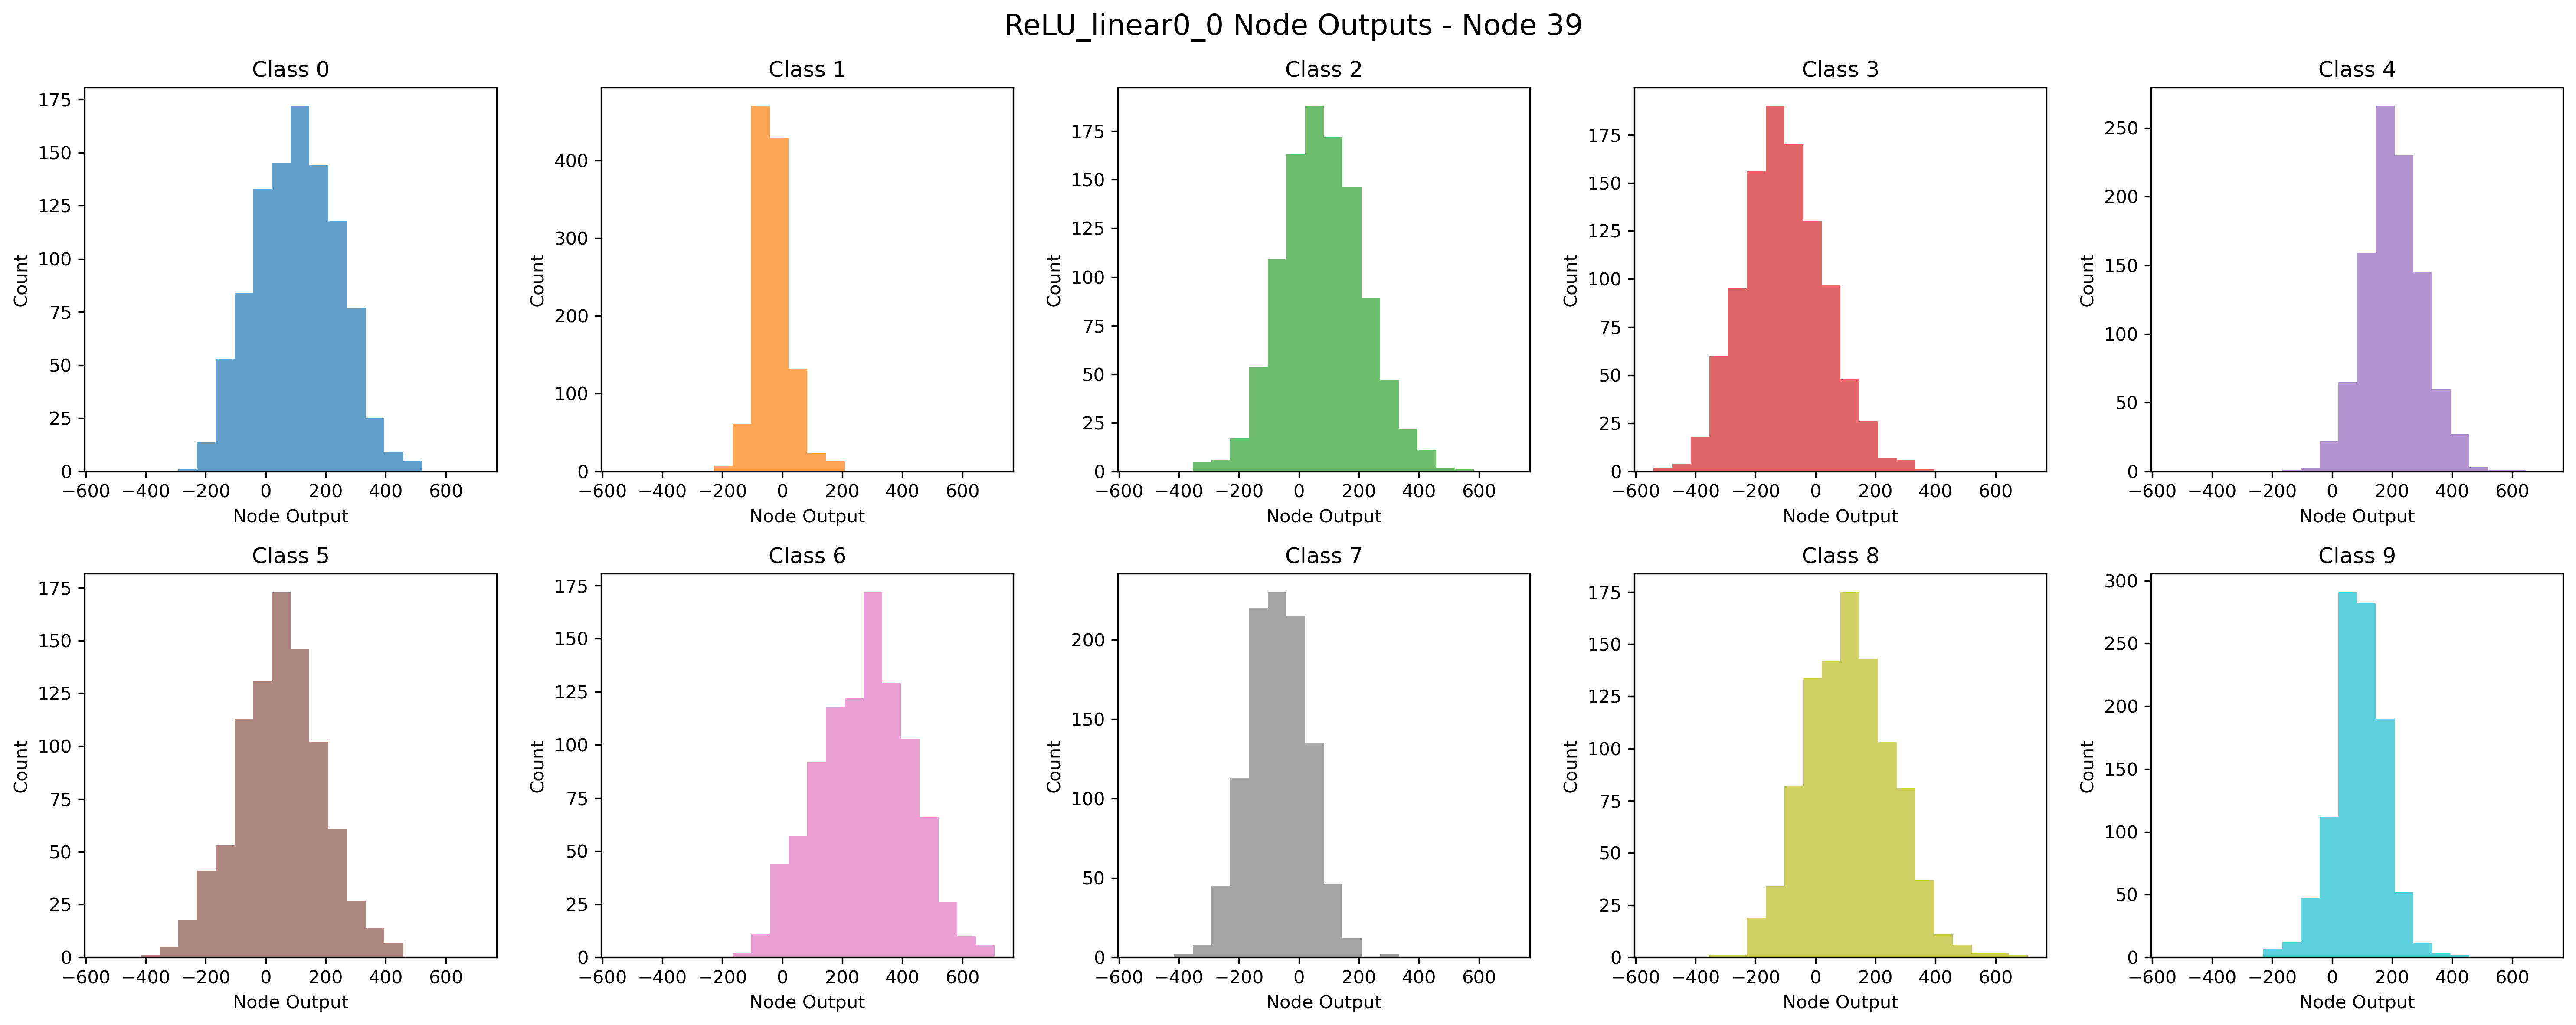
\includegraphics[width=0.4\textwidth]{images/distance_distribution}
    \caption{Class distributions in the latent space show overlapping clusters with varying statistical properties. Each class exhibits distinct characteristics (mean, variance, skewness), with overlap patterns varying across different linear projections - typical behavior for non-linearly separable data.}
    \label{fig:distance_distribution}
\end{figure}
The first linear layer's outputs form a 128-dimensional latent space, where the second layer defines a hyperplane $y=Wx+b$ ($b=0$). While traditional analysis views hyperplanes as boundaries that separate clusters, our distance-based interpretation focuses on how hyperplanes intersect clusters to define prototypes. The hyperplane is uniquely defined by 128 points: 127 points on the decision boundary (representing learned prototypes within clusters), the origin (due to $b=0$), and one point outside the latent space. These intersections with clusters determine the hyperplane's orientation and thus how the network measures distances to prototypes for classification.In this latent space, we define two important points for each class $c$: an optimal center $z_c$ that minimizes intra-class distances while maximizing inter-class distances, and its counterpart $z_{\neg c}$ that does the opposite. These points, constructed from the first layer's node outputs, represent ideal prototypes within their respective clusters.
When learning a distance representation, the second linear layer's hyperplane attempts to intersect points approximating $z_c$ on its decision boundary. This alignment ensures the target class has minimal activations by positioning the boundary near its ideal center, effectively identifying classes based on their proximity to these centers.
When learning an intensity representation, the second linear layer's hyperplane attempts to intersect points approximating $z_{\neg c}$ on its decision boundary. This alignment ensures the target class has maximal activations by positioning the boundary near the centers of non-target classes, effectively separating classes based on their distance from these "anti-centers."
\subsection{Analysis of ReLU-based Architectures}

\texttt{ReLU2} failed catastrophically ($47.20\% \pm 12.00\%$) due to widespread node death in its output layer: $33.00\%$ of nodes were permanently inactive and $53.50\%$ activated for less than 5\% of inputs. This failure stems from attempting to learn a disjunctive distance representation while constrained by intensity-based learning. Since non-target classes comprise 90\% of the data for any classification decision, the network drives most pre-activations negative to minimize non-target activations.

The dead node collapse emerges from a compounding effect: when classes overlap in the latent space, minimizing activations for non-target classes ($\neg c$) inevitably affects the target class ($c$) as well. Since each class comprises only 10\% of the data, the optimization overwhelmingly prioritizes minimizing non-target activations (90\% of cases) over preserving activations for the target class (10\% of cases). As a result, pre-activations for both target and non-target classes are driven negative, which the second ReLU then zeros out, leading to widespread dead nodes.

In contrast, \texttt{ReLU2-Neg} achieves near-baseline performance ($94.93\% \pm 0.15\%$) by building a conjunctive distance representation. It positions hyperplanes so that class $c$ points have negative pre-activations (centered around $z_c$), which ReLU converts to zero. Crucially, this also applies to all classes with even smaller pre-activations (i.e., those positioned to the left of $z_c$ in the projected space, as shown in Figure~\ref{fig:distance_distribution}). Since ReLU zeros out everything below the target class, the network must rely on the decorrelation of these classes across different hyperplane projections to prevent them from overlapping with the target class. The diverse projections in the latent space ensure this decorrelation, allowing the target class to maintain minimal activation while maximizing $\neg c$.

\subsection{Analysis of Abs-based Architectures}

Unlike ReLU, Abs networks cannot produce dead nodes. Instead of zeroing out negative values, Abs folds them to the positive side, ensuring all nodes remain active. Under our distance metric theory—where zero activation signifies maximum feature membership—this architectural difference leads to distinct feature representations. 

In ReLU networks, maximum feature membership extends to all input regions producing negative pre-activations, creating broader feature sets. In contrast, Abs networks achieve maximum membership only at exact decision boundary points, resulting in more focused feature sets. Since the minimum activation can correspond to either $z_c$ or $z_{\neg c}$, Abs networks provide a more direct encoding of distances to learned prototypes or anti-prototypes.

While \texttt{Abs2} performed well ($95.35\% \pm 0.17\%$), its distance-learning counterpart, \texttt{Abs2-Neg}, suffered a notable accuracy drop ($90.08\% \pm 2.56\%$) with significantly higher variance. What explains this unexpected performance gap?

We theorize that \texttt{Abs2-Neg} underperformance may be related to the clustered nature of MNIST. This dataset's distinct clusters might lead to the existence of a single, highly optimal prototype point, $z_c$, for each class. An output hyperplane in \texttt{Abs2-Neg} must pass through that optimal prototype $z_c$ and 127 additional linearly independent points. If a single, dominant $z_c$ exists, the remaining points must be suboptimal, potentially lying closer to non-target class distributions. This constraint could lead to misclassifications and higher variance. The development of \texttt{OffsetL2}, which explicitly models a single prototype per class, was motivated by this hypothesis.

In contrast, \texttt{Abs2} constructs its hyperplane by selecting $z_{\neg c}$, the centers of non-target classes, for each latent dimension. Since each dimension can be aligned with any of the nine non-target classes, \texttt{Abs2} has a vast combinatorial space of possible hyperplane configurations ($9^{128}$ choices). This flexibility allows it to compensate for suboptimal points in some dimensions by making better choices in others. As a result, \texttt{Abs2} can achieve robust class separation, explaining its higher accuracy and lower variance compared to \texttt{Abs2-Neg}.

\subsection{Validation Through Additional Experiments}

Our theory about the \texttt{Abs2-Neg} performance drop suggests that a layer designed to explicitly represent the distance to a single optimal point might correct the performance difference. To address the limitations of \texttt{Abs2-Neg}, where the need for multiple non-optimal intersection points hampered performance, we propose a layer called OffsetL2 that computes the weighted L2 distance from a single learned reference point $\mu$:

\[
y_i = || \alpha_i \odot (x - \mu_i) ||_2
\]

OffsetL2 directly implements our geometric intuition by explicitly learning a single optimal reference point, $\mu_i$, for each class, corresponding to the hypothesized ideal prototype $z_c$. The learnable weight vector $\alpha_i$ modulates the importance of each dimension in the distance calculation, providing greater flexibility. This approach contrasts with \texttt{Abs2-Neg}, which implicitly discovers prototypes through hyperplane positioning.

When combined with LogSoftmax, OffsetL2 shows interesting connections to established architectures:

\begin{table}[H]
    \centering
    \footnotesize
    \begin{tabular}{lc}
        \toprule
        \textbf{Method} & \textbf{Equation} \\
        \midrule
        OffsetL2 + LogSoftmax & $ y_i = \exp(-||\alpha_i \odot (x - \mu_i) ||_2) $ \\  
        Traditional RBF & $ y_i = \exp(-0.5 (\text{precision}_i (x - \mu_i)^2)) $ \\  
        Mahalanobis + LogSoftmax & $ y_i = \exp(-||\text{precision}_i v_i (x - \mu_i)||_2) $ \\  
        \bottomrule
    \end{tabular}
    \caption{Comparison of OffsetL2 with related distance-based methods.}
    \label{tab:comparison_offsetl2}
\end{table}

When preceded by a linear layer, OffsetL2 becomes functionally equivalent to the PCA-based Mahalanobis distance, where the linear layer learns principal components ($V$) and OffsetL2 learns the scaling ($\Lambda^{-1/2}$) and mean ($\mu$). This strong connection between OffsetL2, RBF networks, and Mahalanobis distance further reinforces its theoretical grounding.

To evaluate OffsetL2, we introduced four new models: \texttt{ReLU-L2}, \texttt{ReLU-L2-Neg}, \texttt{Abs-L2}, and \texttt{Abs-L2-Neg}. Training was extended to 50,000 epochs after observing that models had not fully converged at 5,000 epochs.


\begin{table}[H]
    \centering
    \footnotesize
    \begin{tabular}{lcc}
    \toprule
    \textbf{Model} & \textbf{Accuracy (\%)} & \textbf{Std Dev (\%)} \\
    \midrule
    % Baseline Models
    ReLU\_Bias & 96.62 & 0.17 \\
    ReLU2\_Bias & 56.31 & 19.31 \\
    ReLU2\_Neg & 96.46 & 0.17 \\
    Abs\_Bias & 95.87 & 0.22 \\
    Abs2\_Bias & 95.95 & 0.17 \\
    Abs2\_Neg\_Bias & 92.25 & 2.07 \\
    \midrule
    % OffsetL2 Models
    ReLU-L2 & 97.33 & 0.13 \\
    ReLU-L2-Neg & 97.36 & 0.14 \\
    Abs-L2 & 97.61 & 0.07 \\
    Abs-L2-Neg & 97.56 & 0.09 \\
    \bottomrule
    \end{tabular}
    \caption{Performance metrics across all models with extended training (50,000 epochs), averaged over 20 runs.}
    \label{tab:extended_training}
\end{table}

The results demonstrate several key findings:

1. The performance gap between normal and negated variants disappeared, supporting our theory about explicit prototype learning.
2. \texttt{ReLU-L2} avoided the catastrophic failure of \texttt{ReLU2\_Bias}.
3. OffsetL2 architectures significantly outperformed baselines, with \texttt{Abs-L2} models achieving $\sim 97.6\%$ accuracy.
4. All OffsetL2 models exhibited remarkably low variance ($\leq 0.14\%$).

These findings validate our theoretical framework: by explicitly modeling geometric constraints through direct distance calculations, OffsetL2 not only improves accuracy but also stabilizes training. The convergence in performance between normal and negated variants provides strong empirical validation of our core hypothesis—explicitly modeling distances to learned prototypes leads to more robust and accurate learning.

Our results, combined with geometric analysis, suggest a fundamental shift in how neural network representations should be conceptualized. Moving beyond the traditional intensity-based paradigm, these findings highlight the power of statistical distance metrics and geometric constraints, paving the way for new architectural advances in deep learning.

\section{Conclusion}

This work advances our understanding of neural networks by revealing their fundamental nature to learn statistical distance metrics. Through systematic experimentation, theoretical analysis, and the development of a novel architecture, we present three key contributions.

First, we demonstrate that neural networks naturally learn statistical distance metrics, with their performance shaped by how effectively architectures support this fundamental behavior. Performance differences across six architectural variants arise not from inherent biases but from how effectively architectures navigate these constraints in the feature space. This insight redefines the role of architecture in determining representational preferences.

Second, we provide theoretical and empirical evidence for why certain architectures succeed or fail under specific constraints. The catastrophic failure of ReLU2 ($47.20\%$ accuracy) reveals how intensity-based constraints can create untenable optimization landscapes, especially when inputs must align with decision boundaries under high-dimensional imbalance. Conversely, the performance gap between Abs2 ($95.35\%$ accuracy) and Abs2-Neg ($90.08\%$ accuracy) highlights the critical importance of combinatorial flexibility in leveraging multiple optimal separation points across high-dimensional spaces. These examples illustrate how geometric interactions, not intrinsic properties of activation functions, drive network performance.

Third, we introduce OffsetL2, a novel architecture explicitly incorporating Mahalanobis distance calculations. OffsetL2 directly models the geometric principles uncovered in our analysis, achieving state-of-the-art performance ($97.61\%$ accuracy) with remarkable stability ($\pm0.07\%$ standard deviation) across all variants. This success validates our theoretical framework linking neural network representations to statistical distance measures and demonstrates the power of explicitly incorporating geometric constraints into network design.

These findings have significant implications for neural architecture design. Rather than evaluating architectural components solely based on biological motivation or gradient flow, we propose a geometric perspective: analyzing the interaction between activation functions, architectural components, and the constraints of the feature space. This approach provides a principled foundation for designing more robust, interpretable, and efficient networks. 

Looking ahead, future work should explore the application of these geometric principles to deeper architectures and more complex tasks, such as natural language processing, reinforcement learning, and unsupervised representation learning. Additionally, integrating OffsetL2-like designs into large-scale systems may yield new insights into the scalability and generalizability of these ideas.

In conclusion, this research underscores the value of viewing neural networks through the lens of geometric and statistical principles. By explicitly modeling these constraints, as demonstrated with OffsetL2, we can improve performance, stability, and interpretability, paving the way for the next generation of principled machine learning architectures.


\bibliographystyle{plain}
\bibliography{references}

\end{multicols}
\end{document}